\subsection{\textbf{Clean Accuracy and Evaluation Units}}
\CurrentPooledResultsTable
\CurrentComparisonTable
\CurrentRawResultsTable
\CurrentAdaptiveCalibrationTable
The frozen shared model achieves official clean capped RMSE 12.0080 and MAE 8.5224 cycles across 707 endpoint engines. Original pooled revision 2 had RMSE 12.1062 on the reused official benchmark. Internal clean RMSE is 13.2974; its 484 prefixes belong to 71 engines and are dependent within engine. These comparisons describe completed runs, rather than an independent confirmatory test.
The immediate preserved fine-tuned source had official RMSE 11.9415; Table~\ref{tab:current_comparison} reports that comparison as well, including any regressions. Validation guards and the held selection-tail objective fixed the current model before these test values were read.
\begin{figure*}[tp]\centering
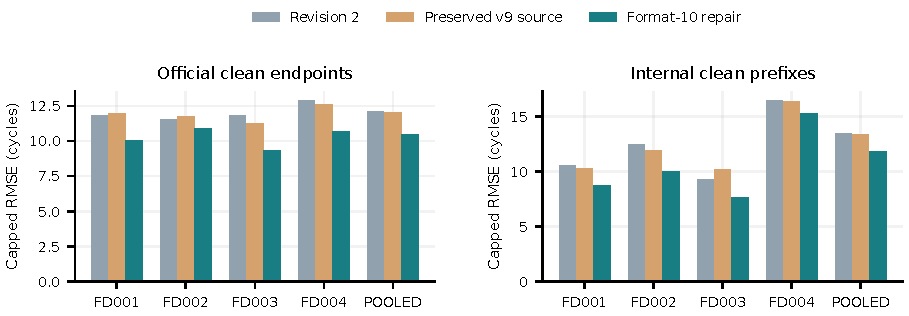
\includegraphics[width=\textwidth]{paper_assets/current_pooled_clean.pdf}
\caption{Clean capped RMSE for the frozen current model, its immediate preserved source, and original pooled revision 2. Each is one training-seed pipeline; no across-training-seed uncertainty is implied. Internal values use a fixed causal prefix grid.}\label{fig:pooled_clean}
\end{figure*}
\subsection{\textbf{Structured-Fault Robustness}}
At severity 0.2, mean pooled official stuck-fault RMSE is 15.0767 cycles over three corruption realizations. Averaging all declared stuck severities and realizations instead gives 17.6636; these summaries must not be interchanged. Fig.~\ref{fig:pooled_faults} exposes severity dependence on the pooled fleet and the multi-regime subsets. Corruptions preserve original RUL labels and do not represent recorded aircraft sensor incidents.
\begin{figure*}[tp]\centering
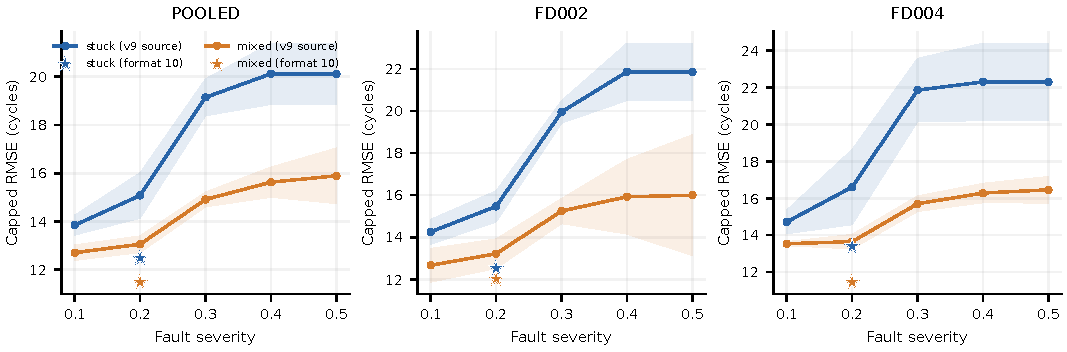
\includegraphics[width=\textwidth]{paper_assets/current_pooled_faults.pdf}
\par\smallskip
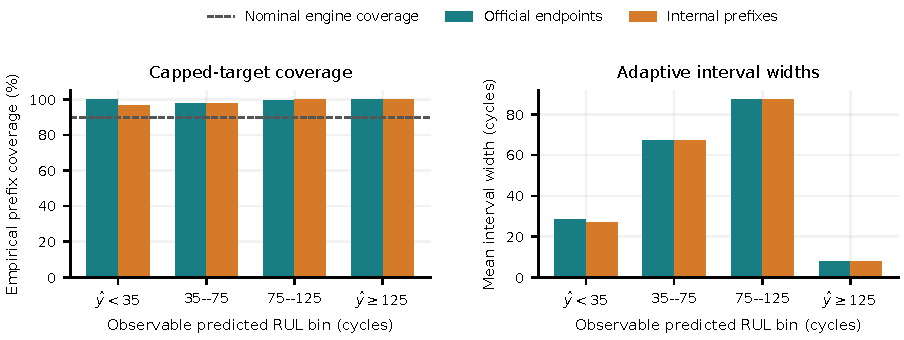
\includegraphics[width=\textwidth]{paper_assets/current_pooled_calibration.pdf}
\caption{Top: official capped-target robustness under structured faults; curves are means and bands are sample standard deviations over three corruption replicates of one frozen model, not training seeds or fleet confidence intervals. Bottom: empirical clean coverage and mean interval width grouped by observable predicted RUL. Grouped coverage is descriptive and does not establish conditional coverage for a realized engine or life stage. The simultaneous calibration score spans all bins for each engine.}\label{fig:pooled_faults}\label{fig:pooled_calibration}
\end{figure*}
\subsection{\textbf{Calibration and Healthy-Sensor Impact}}
Empirical clean coverage is 99.29\% on official endpoints and 98.97\% on internal prefixes. Internal whole-engine coverage over the evaluated grid is 95.77\%, a different unit from prefix coverage and from every-cycle trajectory coverage. Nominal coverage is 90\%, conditional on the stated exchangeability assumptions. The complete recovery matrix is accepted with worst pooled-context intact original-linear RMSE 0.00983; this is a sensor displacement diagnostic, not a RUL accuracy guarantee.
\subsection{\textbf{Broadband Sensor Noise and Channel Dropout}}
\newcommand{\CurrentNoiseTable}{%
\begin{table*}[!t]
\caption{Frozen-artifact accuracy under broadband sensor noise and channel dropout.}
\label{tab:noise}
\centering\footnotesize
\setlength{\tabcolsep}{3pt}
\begin{tabular}{lrrrrr}
\toprule
Noise & Official RMSE & Official MAE & Cov. (\%) & Internal RMSE & Cov. (\%) \\
\midrule
none & 12.01 & 8.52 & 99.3 & 13.30 & 99.0 \\
5\% & 12.05 & 8.60 & 99.3 & 13.37 & 99.0 \\
10\% & 12.17 & 8.62 & 99.2 & 13.55 & 99.2 \\
20\% & 12.37 & 8.76 & 98.9 & 13.84 & 98.8 \\
30\% & 12.67 & 9.04 & 99.0 & 14.29 & 98.8 \\
50\% & 13.68 & 9.97 & 99.2 & 15.44 & 97.9 \\
2\% cells & 11.96 & 8.56 & 99.6 & 13.37 & 99.0 \\
5\% cells & 12.23 & 8.77 & 99.2 & 13.54 & 99.0 \\
\bottomrule
\end{tabular}
\par\vspace{2pt}
\begin{minipage}{\textwidth}\scriptsize Rows 1--6 add per-channel Gaussian noise; the level is a multiple of the fitting-only within-regime sensor scale. Rows 7--8 instead drop whole cells at zero added noise. Settings and speed commands are unperturbed. Noise is applied after model freeze; no weight, threshold, corrector or interval radius was fitted on these levels. Coverage is empirical clean endpoint/prefix coverage under the frozen radius, not a new guarantee.\end{minipage}
\end{table*}
}

\CurrentNoiseTable
The structured protocol models failures confined to related channels. Real
acquisition also carries broadband noise on every channel at once and occasional
missing cells. We therefore add an independent measurement layer that perturbs
raw sensor readings before the frozen fitting-only scaler: per-channel Gaussian
noise scaled to the within-regime sensor scale, plus independent cell dropouts.
Settings and speed commands stay untouched, and the layer is applied only after
freeze, so no weight, detector threshold, corrector or interval radius was fitted
on it. Levels are nested: one per-engine draw is scaled, so a sweep is paired
rather than resampled.

Table~\ref{tab:noise} shows graceful degradation. At 20\% of the within-regime
scale, pooled official RMSE moves from \CurrentNoiseOfficialZero{} to
\CurrentNoiseOfficialTwenty{} cycles, an increase of 3.0\%, and empirical coverage
remains \CurrentNoiseCoverageTwenty{}\%. At 50\% it is
\CurrentNoiseOfficialFifty{} cycles with \CurrentNoiseCoverageFifty{}\% coverage.
The internal partition follows the same pattern, from \CurrentNoiseHeldoutZero{}
to \CurrentNoiseHeldoutFifty{}. Modest dropout is not harmful: dropping 2\% of
cells leaves pooled official RMSE at \CurrentNoiseDropoutTwo{}, and 5\% gives
\CurrentNoiseDropoutFive{}. These are sensitivity measurements of one frozen
artifact, not a claim that any level matches a measured sensor specification.

\subsection{\textbf{Comparison with the Supplied Studies}}
\newcommand{\CurrentLiteratureTable}{%
\begin{table*}[!t]
\caption{Reported C-MAPSS results at the 125-cycle target against the supplied studies.}
\label{tab:literature}
\centering\footnotesize
\setlength{\tabcolsep}{3pt}
\begin{tabular}{lrrrr}
\toprule
Model & FD001 & FD002 & FD003 & FD004 \\
\midrule
GRACE-RUL (one shared model, no subset label) & \textbf{11.93} & \textbf{11.77} & \textbf{11.25} & \textbf{12.57} \\
Hybrid CNN--GRU (reported, five repeats) & 13.1 & 16.8 & 14.5 & 18.9 \\
TRANS-D3 (reported) & 1.66 & 13.23 & 6.61 & 12.26 \\
Best third-party baseline (reported) & 10.61 (STAR) & 13.47 (STAR) & 10.71 (STAR) & 15.86 (DLformer) \\
Reported value ahead of GRACE-RUL & TRANS-D3 1.66 & none & TRANS-D3 6.61 & TRANS-D3 12.26 \\
Position among third-party baselines (proposed row excluded) & 6 & 1 & 3 & 1 \\
\bottomrule
\end{tabular}
\par\vspace{2pt}
\begin{minipage}{\textwidth}\scriptsize Reported columns are transcribed from the cited papers and are not recomputed here. Rank counts only third-party baselines, so a proposed row cannot define its own benchmark. The penultimate row names every reported value still ahead of this work, including the TRANS-D3 proposed row where it applies; on FD004 this work is second overall, not first. This work is one shared model without a subset label, whereas the compared entries are subset-specific. Official C-MAPSS tests were inspected in earlier development, so all values are exploratory rather than a pristine holdout.\end{minipage}
\end{table*}
}

\CurrentLiteratureTable
Table~\ref{tab:literature} transcribes the reported values of the supplied
studies. This work is first on FD002 among every reported row, second on FD004
behind the reported TRANS-D3 value of 12.26, third on FD003 among third-party
baselines, and \CurrentRankFdA{}th on FD001. It is not first on FD004 and no
such claim is made. The hybrid CNN--GRU study reports
13.1, 16.8, 14.5 and 18.9, so this model improves every subset by 1.17 to 6.33
cycles at a comparable 125-cycle target.

Two qualifications matter more than the ordering. First, the compared entries are
subset-specific models, whereas this work uses one shared model without a subset
label, so the comparison is not budget-matched in the harder direction. Second,
the TRANS-D3 FD001 and FD003 values of 1.66 and 6.61 lie far below every
third-party entry in the same table, whose best values are \CurrentBestFdA{}
and \CurrentBestFdB{}; no capped C-MAPSS protocol in this study reaches them, so they are
retained for completeness rather than treated as a reproducible target. The
partial-failure study reports a single pooled fault-conditioned RMSE of
\CurrentPaperBOfficial{} with unspecified channel coverage and severity, which is
not decomposable by subset and is therefore not entered as a per-subset cell.

\begin{figure*}[tp]\centering
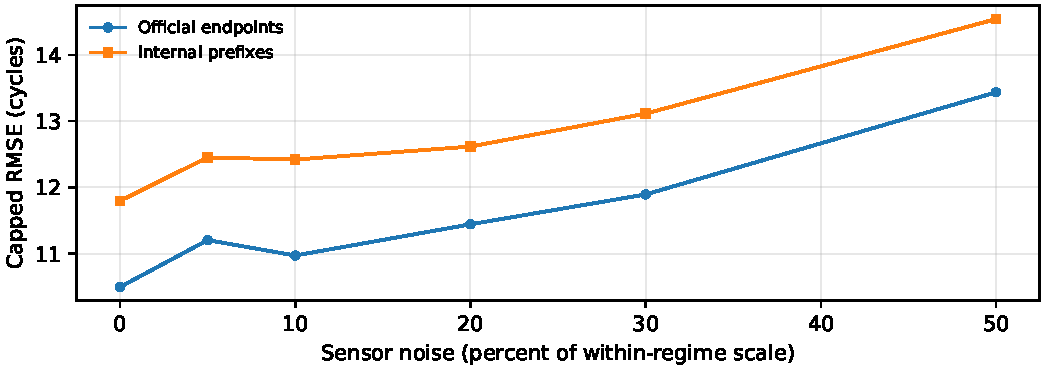
\includegraphics[width=0.86\textwidth]{paper_assets/current_noise_curves.pdf}
\caption{Capped RMSE of the frozen artifact against broadband sensor noise. Every point is one evaluation of the same weights, scaler and interval radius, with the bounded corrector disabled; levels are paired draws, not independent realizations or training seeds.}
\label{fig:noise_curves}\end{figure*}

\subsection{\textbf{Component Contribution and Interval Width}}
\newcommand{\CurrentAblationTable}{%
\begin{table*}[!t]
\caption{Post-freeze component ablation of one unchanged artifact.}
\label{tab:ablation}
\centering\footnotesize
\setlength{\tabcolsep}{4pt}
\begin{tabular}{lrrrrr}
\toprule
Condition & Full & $-$Recovery & Neither & Cov. (\%) & Width \\
\midrule
clean & 10.50 & 10.64 & 10.64 & 99.7 & 89.5 \\
intermittent & 10.71 & 10.90 & 10.90 & 99.7 & 89.7 \\
outage & 11.19 & 12.67 & 12.67 & 99.7 & 89.3 \\
block & 10.76 & 11.47 & 11.47 & 99.7 & 89.3 \\
noise & 11.10 & 11.20 & 11.20 & 99.7 & 90.2 \\
bias & 10.93 & 11.05 & 11.05 & 99.7 & 90.0 \\
drift & 10.80 & 10.91 & 10.91 & 99.7 & 89.9 \\
stuck & 12.49 & 22.09 & 22.09 & 99.3 & 90.5 \\
mixed & 11.48 & 14.28 & 14.28 & 99.6 & 89.7 \\
\bottomrule
\end{tabular}
\par\vspace{2pt}
\begin{minipage}{\textwidth}\scriptsize All columns use the same weights, scaler, detector thresholds and interval radius; only the inference switches differ. Fault rows average three corruption replicates, clean has none. Nothing was selected, removed or retuned from these values, and the deployed artifact is unchanged. The corrector is disabled in format 10, so a separate $-$Corrector column would be identical to Full. Coverage and mean width are for the full path under the frozen radius. Official benchmarks were inspected in earlier development, so this is a diagnostic, not a holdout.\end{minipage}
\end{table*}
}

\CurrentAblationTable
Table~\ref{tab:ablation} separates what the frozen artifact actually gains from
its parts. The guarded recovery path is the only component with a material
effect, and only under persistent faults: stuck-fault RMSE falls from
\CurrentAblationStuckBypass{} to \CurrentAblationStuckFull{} cycles
(\CurrentAblationStuckGain{}) at severity 0.2, the gain stays between
\CurrentAblationStuckGainHigh{} and \CurrentAblationStuckGainLow{} across
severities 0.1--0.5, and mixed faults improve by
\CurrentAblationMixedGain{}. Outage and block faults gain
\CurrentAblationOutageGain{} and \CurrentAblationBlockGain{} cycles,
respectively. Broadband noise gains only \CurrentAblationNoiseGain{} cycles,
consistent with recovery targeting persistent abnormal readings rather than
additive measurement error. On clean endpoints the full path gives
\CurrentAblationCleanFull{} against \CurrentAblationCleanPlain{} for the
branch-fusion predictor with neither intervention, so the recovery path is not
free when no fault is present.

The bounded observable corrector is disabled in format 10: its exported bound is
zero, so removing it changes RMSE by \CurrentAblationCorrectorDelta{} cycles by
construction. The source artifact's earlier null ablation, where removal changed
RMSE by at most 0.02 cycles and never for the worse, motivated this choice. No
corrector adjustment is present in the reported RUL, and the manuscript makes no
claim that the corrector improves accuracy.

The same table pairs coverage with sharpness. The mean clean official interval is
\CurrentAblationWidth{} cycles wide against a 125-cycle target, so
\CurrentAblationCoverage{}\% empirical coverage at this radius is driven by width
rather than by accurate point prediction. Coverage must therefore be read
alongside width, and neither establishes conditional coverage for a realized
engine. Component selection was frozen before these values were read; the table
is a post-freeze diagnostic and the deployed artifact is unchanged.

\newcommand{\CurrentDetectorTable}{%
\begin{table*}[!t]
\caption{Held-validation detector operating point at severity 0.2.}
\label{tab:detector}
\centering\footnotesize
\setlength{\tabcolsep}{3pt}
\begin{tabular}{llrrr}
\toprule
Family & Scope & F1 & Recall & False positive (\%) \\
\midrule
clean & none & n/a & n/a & 0.03 \\
intermittent & missing & n/a & n/a & 0.05 \\
outage & missing & n/a & n/a & 0.00 \\
block & missing & n/a & n/a & 0.03 \\
noise & finite & 0.42 & 0.27 & 0.20 \\
bias & finite & 0.47 & 0.31 & 0.13 \\
drift & finite & 0.38 & 0.24 & 0.12 \\
stuck & finite & 0.66 & 0.55 & 0.40 \\
mixed & finite & 0.51 & 0.36 & 0.14 \\
\bottomrule
\end{tabular}
\par\vspace{2pt}
\begin{minipage}{\textwidth}\scriptsize Thresholds are frozen deployment buffers at the 5\% per-channel/context intact false-positive ceiling. Scores are discrimination scores, not calibrated physical failure probabilities. Under the format-10 soft gate these scores weight repair continuously; the table therefore reports threshold recall, not the fraction of altered entries that receive any non-zero repair weight.\end{minipage}
\end{table*}
}
\newcommand{\CurrentRecoveryTable}{%
\begin{table*}[!t]
\caption{Post-freeze recovery and detection benchmark by fault family.}
\label{tab:recovery}
\centering\footnotesize
\setlength{\tabcolsep}{3pt}
\begin{tabular}{llrrrrrr}
\toprule
Family & Scope & F1 & Recall & Reconst. RMSE & Intact disp. & False repair (\%) & Cov. (\%) \\
\midrule
clean & none & n/a & n/a & n/a & 0.017 & 0.0 & 98.4 \\
intermittent & missing & n/a & n/a & 0.46 & 0.021 & 0.1 & 98.5 \\
outage & missing & n/a & n/a & 0.46 & 0.011 & 0.0 & 98.4 \\
block & missing & n/a & n/a & 0.45 & 0.019 & 0.0 & 98.6 \\
noise & finite & 0.42 & 0.27 & 0.22 & 0.019 & 0.2 & 98.4 \\
bias & finite & 0.47 & 0.31 & 0.26 & 0.022 & 0.1 & 98.5 \\
drift & finite & 0.38 & 0.24 & 0.19 & 0.020 & 0.1 & 98.7 \\
stuck & finite & 0.66 & 0.55 & 1.99 & 0.023 & 0.4 & 97.6 \\
mixed & finite & 0.51 & 0.36 & 0.47 & 0.015 & 0.1 & 98.5 \\
\bottomrule
\end{tabular}
\par\vspace{2pt}
\begin{minipage}{\textwidth}\scriptsize Detection, false repair and intact displacement use the held selection recovery audit at severity 0.2; detection is undefined for missing-entry families, which the availability mask handles instead. Reconstruction and displacement are original-linear sensor units. Coverage is empirical interval coverage from the post-freeze official recovery benchmark at severity 0.2, where available. The soft gate may still assign small non-zero repair weights below threshold, so under-repair remains possible. Nothing was tuned on these values.\end{minipage}
\end{table*}
}
\subsection{\textbf{Detector Operating Characteristics}}
\CurrentDetectorTable
Table~\ref{tab:detector} makes the detector limitation explicit. Clean false
positives are 0.0322\% of intact entries, but finite-fault recall
is only 0.24 for drift,
0.31 for bias, 0.27 for
noise, and 0.55 for stuck. Recall is low in every
finite family, so the deployed path misses many genuine deviations rather than
over-repairing healthy cells.
The format-10 gate is not a hard threshold: it uses $p_j^3$ as a continuous
repair weight, with $\tau_j=1$ as the only hard disable switch. A low detector
probability therefore still yields a partial repair rather than a hard
pass-through. This mitigates
but does not remove the under-repair failure mode, and the paper makes no
universal recovery claim.

\subsection{\textbf{Recovery and Calibration by Fault Family}}
\CurrentRecoveryTable
Table~\ref{tab:recovery} pairs the detector audit with the complete recovery
matrix. The worst intact displacement is 0.02521
original-linear units, and the worst single-window intact RMSE is
0.06907. Stuck faults are the easiest finite
family to flag (F1 0.66) but still the hardest to
reconstruct, consistent with a held value being ambiguous rather than out of
range. Clean official coverage is 98.4\%; under
severity-0.2 stuck and mixed faults it is
97.6\%
and 98.5\%, respectively.
All 41 declared contexts completed and passed their
intact-cell guards.

\subsection{\textbf{Computational Cost}}
\newcommand{\CurrentEfficiencyTable}{%
\begin{table*}[!t]
\caption{Post-freeze computational cost of the exported artifact.}
\label{tab:efficiency}
\centering\footnotesize
\setlength{\tabcolsep}{3pt}
\begin{tabular}{lrl}
\toprule
Metric & Value & Scope \\
\midrule
Trainable parameters & 348,976 & whole artifact \\
Parameters: detector / generator / predictor / corrector & 37,909 / 176,533 / 132,325 / 2,209 & per module \\
Float32 weight size & 1.33 MB & weights only \\
Multiply-accumulates, full path & 9.6 M & one 70-cycle window \\
Multiply-accumulates, bypass & 6.9 M & one 70-cycle window \\
Latency, full path & 5.40 ms & single window, median \\
Latency, bypass & 2.62 ms & single window, median \\
Latency, plain predictor & 2.67 ms & single window, median \\
Throughput & 10184 engines/s & batch 64, full path \\
Fleet pass & 3.82 s & 707 engines, one window each \\
Process peak memory & 1813 MB & interpreter and torch included \\
\bottomrule
\end{tabular}
\par\vspace{2pt}
\begin{minipage}{\textwidth}\scriptsize Wall-clock measurement of one CPU machine, not a hardware-independent claim; multiply-accumulates are a complexity proxy for supported operations only. The recovery path costs about 106\% latency over bypass and buys the stuck-fault gain in Table~\ref{tab:ablation}. Peak memory includes the Python and PyTorch interpreter, whose baseline is reported in the saved record.\end{minipage}
\end{table*}
}

\CurrentEfficiencyTable
The artifact is small: \CurrentParams{} parameters, 1.33 MB of
float32 weights, and 9.6 M multiply-accumulates
per window. A single-window forward pass takes
5.4 ms on this CPU; the recovery path adds
about 106\%
latency over bypass, which is the price of the stuck-fault gain rather than an overhead to hide.
Batched throughput reaches 10184 engines per
second, so the full 707-engine benchmark evaluates in
3.8 s at batch one. These are wall-clock numbers from
one machine; latency and memory are not hardware-independent and the tables report
no energy measurement.

\subsection{\textbf{Previously Inspected FD004 Engine 179}}
This case is a post-freeze diagnostic, excluded from the current selection objective. At cycle 240 the model predicts 7.440 against capped target 125 (raw RUL 195); its capped interval is [0.000, 22.581]. At cycle 270 it predicts 114.282. Aggregate coverage cannot establish that this particular prediction is accurate or covered. Raw settings at cycles 240 and 245 are [10.0067, 0.2516, 100] and [20.0005, 0.7, 100], respectively, and correspond to different fitted regimes. Consequently the earlier identical-setting physical-excursion explanation is unsupported. The local branch uses 30 cycles and the Transformer uses 70; a local-window-only causal explanation is also incomplete.
\begin{figure*}[tp]\centering
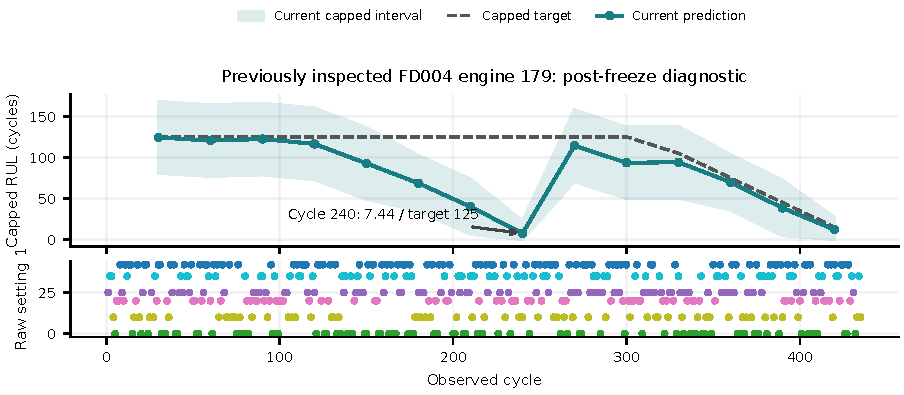
\includegraphics[width=\textwidth]{paper_assets/current_pooled_engine179.pdf}
\caption{Observed failure-case trajectory and operating-setting changes. Predictions and intervals are saved outputs of the frozen current artifact. Colors in the lower panel identify fitted regimes; raw settings are not ground truth about a physical fault cause.}\label{fig:pooled_engine179}
\end{figure*}
\subsection{\textbf{Evidence and Reproducibility Boundaries}}
Point metrics, counts and coverage are recomputed from saved predictions. All manuscript numbers and plotted values are tied to a single completed run, with input/output SHA-256 hashes in \texttt{paper\_assets/current\_provenance.json}; the noise benchmark and the cross-study transcription carry their own record in \texttt{paper\_assets/current\_noise\_provenance.json}. Asset generation performs no model fitting or inference. The source model and earlier audit directories remain preserved; new artifacts use fresh directories. This does not restore independence of previously inspected internal or official benchmark cases. Matched reproductions of the compared methods, repeated training seeds and external fleet validation remain separate requirements.
